\documentclass[]{article}
\usepackage{lmodern}
\usepackage{amssymb,amsmath}
\usepackage{ifxetex,ifluatex}
\usepackage{fixltx2e} % provides \textsubscript
\ifnum 0\ifxetex 1\fi\ifluatex 1\fi=0 % if pdftex
  \usepackage[T1]{fontenc}
  \usepackage[utf8]{inputenc}
\else % if luatex or xelatex
  \ifxetex
    \usepackage{mathspec}
  \else
    \usepackage{fontspec}
  \fi
  \defaultfontfeatures{Ligatures=TeX,Scale=MatchLowercase}
\fi
% use upquote if available, for straight quotes in verbatim environments
\IfFileExists{upquote.sty}{\usepackage{upquote}}{}
% use microtype if available
\IfFileExists{microtype.sty}{%
\usepackage{microtype}
\UseMicrotypeSet[protrusion]{basicmath} % disable protrusion for tt fonts
}{}
\usepackage[margin=1in]{geometry}
\usepackage{hyperref}
\hypersetup{unicode=true,
            pdftitle={Class 6 Homework},
            pdfauthor={Erica Birkholz},
            pdfborder={0 0 0},
            breaklinks=true}
\urlstyle{same}  % don't use monospace font for urls
\usepackage{color}
\usepackage{fancyvrb}
\newcommand{\VerbBar}{|}
\newcommand{\VERB}{\Verb[commandchars=\\\{\}]}
\DefineVerbatimEnvironment{Highlighting}{Verbatim}{commandchars=\\\{\}}
% Add ',fontsize=\small' for more characters per line
\usepackage{framed}
\definecolor{shadecolor}{RGB}{248,248,248}
\newenvironment{Shaded}{\begin{snugshade}}{\end{snugshade}}
\newcommand{\KeywordTok}[1]{\textcolor[rgb]{0.13,0.29,0.53}{\textbf{#1}}}
\newcommand{\DataTypeTok}[1]{\textcolor[rgb]{0.13,0.29,0.53}{#1}}
\newcommand{\DecValTok}[1]{\textcolor[rgb]{0.00,0.00,0.81}{#1}}
\newcommand{\BaseNTok}[1]{\textcolor[rgb]{0.00,0.00,0.81}{#1}}
\newcommand{\FloatTok}[1]{\textcolor[rgb]{0.00,0.00,0.81}{#1}}
\newcommand{\ConstantTok}[1]{\textcolor[rgb]{0.00,0.00,0.00}{#1}}
\newcommand{\CharTok}[1]{\textcolor[rgb]{0.31,0.60,0.02}{#1}}
\newcommand{\SpecialCharTok}[1]{\textcolor[rgb]{0.00,0.00,0.00}{#1}}
\newcommand{\StringTok}[1]{\textcolor[rgb]{0.31,0.60,0.02}{#1}}
\newcommand{\VerbatimStringTok}[1]{\textcolor[rgb]{0.31,0.60,0.02}{#1}}
\newcommand{\SpecialStringTok}[1]{\textcolor[rgb]{0.31,0.60,0.02}{#1}}
\newcommand{\ImportTok}[1]{#1}
\newcommand{\CommentTok}[1]{\textcolor[rgb]{0.56,0.35,0.01}{\textit{#1}}}
\newcommand{\DocumentationTok}[1]{\textcolor[rgb]{0.56,0.35,0.01}{\textbf{\textit{#1}}}}
\newcommand{\AnnotationTok}[1]{\textcolor[rgb]{0.56,0.35,0.01}{\textbf{\textit{#1}}}}
\newcommand{\CommentVarTok}[1]{\textcolor[rgb]{0.56,0.35,0.01}{\textbf{\textit{#1}}}}
\newcommand{\OtherTok}[1]{\textcolor[rgb]{0.56,0.35,0.01}{#1}}
\newcommand{\FunctionTok}[1]{\textcolor[rgb]{0.00,0.00,0.00}{#1}}
\newcommand{\VariableTok}[1]{\textcolor[rgb]{0.00,0.00,0.00}{#1}}
\newcommand{\ControlFlowTok}[1]{\textcolor[rgb]{0.13,0.29,0.53}{\textbf{#1}}}
\newcommand{\OperatorTok}[1]{\textcolor[rgb]{0.81,0.36,0.00}{\textbf{#1}}}
\newcommand{\BuiltInTok}[1]{#1}
\newcommand{\ExtensionTok}[1]{#1}
\newcommand{\PreprocessorTok}[1]{\textcolor[rgb]{0.56,0.35,0.01}{\textit{#1}}}
\newcommand{\AttributeTok}[1]{\textcolor[rgb]{0.77,0.63,0.00}{#1}}
\newcommand{\RegionMarkerTok}[1]{#1}
\newcommand{\InformationTok}[1]{\textcolor[rgb]{0.56,0.35,0.01}{\textbf{\textit{#1}}}}
\newcommand{\WarningTok}[1]{\textcolor[rgb]{0.56,0.35,0.01}{\textbf{\textit{#1}}}}
\newcommand{\AlertTok}[1]{\textcolor[rgb]{0.94,0.16,0.16}{#1}}
\newcommand{\ErrorTok}[1]{\textcolor[rgb]{0.64,0.00,0.00}{\textbf{#1}}}
\newcommand{\NormalTok}[1]{#1}
\usepackage{graphicx,grffile}
\makeatletter
\def\maxwidth{\ifdim\Gin@nat@width>\linewidth\linewidth\else\Gin@nat@width\fi}
\def\maxheight{\ifdim\Gin@nat@height>\textheight\textheight\else\Gin@nat@height\fi}
\makeatother
% Scale images if necessary, so that they will not overflow the page
% margins by default, and it is still possible to overwrite the defaults
% using explicit options in \includegraphics[width, height, ...]{}
\setkeys{Gin}{width=\maxwidth,height=\maxheight,keepaspectratio}
\IfFileExists{parskip.sty}{%
\usepackage{parskip}
}{% else
\setlength{\parindent}{0pt}
\setlength{\parskip}{6pt plus 2pt minus 1pt}
}
\setlength{\emergencystretch}{3em}  % prevent overfull lines
\providecommand{\tightlist}{%
  \setlength{\itemsep}{0pt}\setlength{\parskip}{0pt}}
\setcounter{secnumdepth}{0}
% Redefines (sub)paragraphs to behave more like sections
\ifx\paragraph\undefined\else
\let\oldparagraph\paragraph
\renewcommand{\paragraph}[1]{\oldparagraph{#1}\mbox{}}
\fi
\ifx\subparagraph\undefined\else
\let\oldsubparagraph\subparagraph
\renewcommand{\subparagraph}[1]{\oldsubparagraph{#1}\mbox{}}
\fi

%%% Use protect on footnotes to avoid problems with footnotes in titles
\let\rmarkdownfootnote\footnote%
\def\footnote{\protect\rmarkdownfootnote}

%%% Change title format to be more compact
\usepackage{titling}

% Create subtitle command for use in maketitle
\newcommand{\subtitle}[1]{
  \posttitle{
    \begin{center}\large#1\end{center}
    }
}

\setlength{\droptitle}{-2em}
  \title{Class 6 Homework}
  \pretitle{\vspace{\droptitle}\centering\huge}
  \posttitle{\par}
  \author{Erica Birkholz}
  \preauthor{\centering\large\emph}
  \postauthor{\par}
  \predate{\centering\large\emph}
  \postdate{\par}
  \date{January 25, 2019}


\begin{document}
\maketitle

\subsection{Simplifying Replicable
Functions}\label{simplifying-replicable-functions}

\begin{Shaded}
\begin{Highlighting}[]
\CommentTok{#Original code}
\KeywordTok{library}\NormalTok{(bio3d)}
\end{Highlighting}
\end{Shaded}

\begin{verbatim}
## Warning: package 'bio3d' was built under R version 3.4.4
\end{verbatim}

\begin{Shaded}
\begin{Highlighting}[]
\NormalTok{s1 <-}\StringTok{ }\KeywordTok{read.pdb}\NormalTok{(}\StringTok{"4AKE"}\NormalTok{) }\CommentTok{# kinase with drug}
\end{Highlighting}
\end{Shaded}

\begin{verbatim}
##   Note: Accessing on-line PDB file
\end{verbatim}

\begin{Shaded}
\begin{Highlighting}[]
\NormalTok{s2 <-}\StringTok{ }\KeywordTok{read.pdb}\NormalTok{(}\StringTok{"1AKE"}\NormalTok{) }\CommentTok{# kinase no drug}
\end{Highlighting}
\end{Shaded}

\begin{verbatim}
##   Note: Accessing on-line PDB file
##    PDB has ALT records, taking A only, rm.alt=TRUE
\end{verbatim}

\begin{Shaded}
\begin{Highlighting}[]
\NormalTok{s3 <-}\StringTok{ }\KeywordTok{read.pdb}\NormalTok{(}\StringTok{"1E4Y"}\NormalTok{) }\CommentTok{# kinase with drug}
\end{Highlighting}
\end{Shaded}

\begin{verbatim}
##   Note: Accessing on-line PDB file
\end{verbatim}

\begin{Shaded}
\begin{Highlighting}[]
\NormalTok{s1.chainA <-}\StringTok{ }\KeywordTok{trim.pdb}\NormalTok{(s1, }\DataTypeTok{chain=}\StringTok{"A"}\NormalTok{, }\DataTypeTok{elety=}\StringTok{"CA"}\NormalTok{)}
\NormalTok{s2.chainA <-}\StringTok{ }\KeywordTok{trim.pdb}\NormalTok{(s2, }\DataTypeTok{chain=}\StringTok{"A"}\NormalTok{, }\DataTypeTok{elety=}\StringTok{"CA"}\NormalTok{)}
\NormalTok{s3.chainA <-}\StringTok{ }\KeywordTok{trim.pdb}\NormalTok{(s3, }\DataTypeTok{chain=}\StringTok{"A"}\NormalTok{, }\DataTypeTok{elety=}\StringTok{"CA"}\NormalTok{) }\CommentTok{#I fixed the error to check against the right plots.}
\NormalTok{s1.b <-}\StringTok{ }\NormalTok{s1.chainA}\OperatorTok{$}\NormalTok{atom}\OperatorTok{$}\NormalTok{b}
\NormalTok{s2.b <-}\StringTok{ }\NormalTok{s2.chainA}\OperatorTok{$}\NormalTok{atom}\OperatorTok{$}\NormalTok{b}
\NormalTok{s3.b <-}\StringTok{ }\NormalTok{s3.chainA}\OperatorTok{$}\NormalTok{atom}\OperatorTok{$}\NormalTok{b}
\KeywordTok{plotb3}\NormalTok{(s1.b, }\DataTypeTok{sse=}\NormalTok{s1.chainA, }\DataTypeTok{typ=}\StringTok{"l"}\NormalTok{, }\DataTypeTok{ylab=}\StringTok{"Bfactor"}\NormalTok{)}
\end{Highlighting}
\end{Shaded}

\includegraphics{Class_6_Homework_files/figure-latex/unnamed-chunk-1-1.pdf}

\begin{Shaded}
\begin{Highlighting}[]
\KeywordTok{plotb3}\NormalTok{(s2.b, }\DataTypeTok{sse=}\NormalTok{s2.chainA, }\DataTypeTok{typ=}\StringTok{"l"}\NormalTok{, }\DataTypeTok{ylab=}\StringTok{"Bfactor"}\NormalTok{)}
\end{Highlighting}
\end{Shaded}

\includegraphics{Class_6_Homework_files/figure-latex/unnamed-chunk-1-2.pdf}

\begin{Shaded}
\begin{Highlighting}[]
\KeywordTok{plotb3}\NormalTok{(s3.b, }\DataTypeTok{sse=}\NormalTok{s3.chainA, }\DataTypeTok{typ=}\StringTok{"l"}\NormalTok{, }\DataTypeTok{ylab=}\StringTok{"Bfactor"}\NormalTok{)}
\end{Highlighting}
\end{Shaded}

\includegraphics{Class_6_Homework_files/figure-latex/unnamed-chunk-1-3.pdf}

\subsection{Create a function based on each step to be taken on one
sample.}\label{create-a-function-based-on-each-step-to-be-taken-on-one-sample.}

\begin{Shaded}
\begin{Highlighting}[]
\CommentTok{#Bfactor has the inputs of a PDB code and which chain to analyze. I would allow the atom type to be selected but it appears C-alpha is the only (most?) relevant one. I would also allow parameters besides Bfactor to be plotted but the pdb table does not appear to contain data best visualized by plotting.  This function plots the Bfactor of each residue in the specific chain of a protein, on a lined scatterplot with marginal secondary structure notation.}
\NormalTok{Bfactor <-}\StringTok{ }\ControlFlowTok{function}\NormalTok{(x, c, t, }\DataTypeTok{na.rm=}\OtherTok{TRUE}\NormalTok{)\{}
\NormalTok{  full <-}\StringTok{ }\KeywordTok{read.pdb}\NormalTok{(x)  }
  \CommentTok{#Read in the protein.}
\NormalTok{  chain <-}\StringTok{ }\KeywordTok{trim.pdb}\NormalTok{(full, }\DataTypeTok{chain=}\NormalTok{c, }\DataTypeTok{elety=}\StringTok{"CA"}\NormalTok{)}
  \CommentTok{#Pull only chain A and atom type C alpha.}
\NormalTok{  bfac <-}\StringTok{ }\NormalTok{chain}\OperatorTok{$}\NormalTok{atom}\OperatorTok{$}\NormalTok{b  }
  \CommentTok{#Store the B factor for each atom in trimmed "chain".}
  \KeywordTok{plotb3}\NormalTok{(bfac, }\DataTypeTok{sse=}\NormalTok{chain, }\DataTypeTok{typ=}\StringTok{"l"}\NormalTok{, }\DataTypeTok{ylab=}\StringTok{"Bfactor"}\NormalTok{)}
  \CommentTok{#Draw standard scatter plot with secondary structure (sse), lines, and a y-axis label.}
\NormalTok{\}}
\CommentTok{#Use that function! View that plot!}
\KeywordTok{Bfactor}\NormalTok{(}\StringTok{"4AKE"}\NormalTok{, }\StringTok{"A"}\NormalTok{)}
\end{Highlighting}
\end{Shaded}

\begin{verbatim}
##   Note: Accessing on-line PDB file
\end{verbatim}

\begin{verbatim}
## Warning in get.pdb(file, path = tempdir(), verbose = FALSE): C:\Users\erica
## \AppData\Local\Temp\RtmpYXg6sv/4AKE.pdb exists. Skipping download
\end{verbatim}

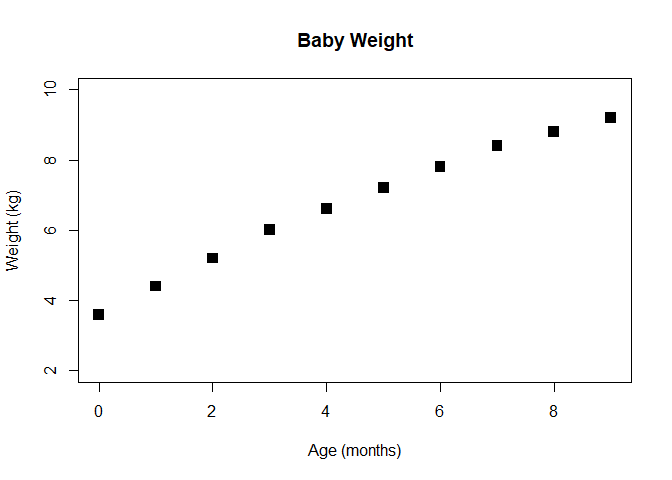
\includegraphics{Class_6_Homework_files/figure-latex/unnamed-chunk-2-1.pdf}

\begin{Shaded}
\begin{Highlighting}[]
\KeywordTok{Bfactor}\NormalTok{(}\StringTok{"1AKE"}\NormalTok{, }\StringTok{"A"}\NormalTok{)}
\end{Highlighting}
\end{Shaded}

\begin{verbatim}
##   Note: Accessing on-line PDB file
\end{verbatim}

\begin{verbatim}
## Warning in get.pdb(file, path = tempdir(), verbose = FALSE): C:\Users\erica
## \AppData\Local\Temp\RtmpYXg6sv/1AKE.pdb exists. Skipping download
\end{verbatim}

\begin{verbatim}
##    PDB has ALT records, taking A only, rm.alt=TRUE
\end{verbatim}

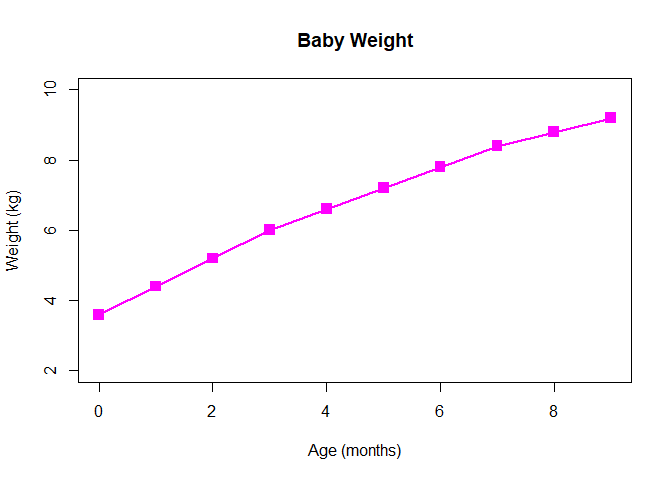
\includegraphics{Class_6_Homework_files/figure-latex/unnamed-chunk-2-2.pdf}

\begin{Shaded}
\begin{Highlighting}[]
\KeywordTok{Bfactor}\NormalTok{(}\StringTok{"1E4Y"}\NormalTok{, }\StringTok{"A"}\NormalTok{)}
\end{Highlighting}
\end{Shaded}

\begin{verbatim}
##   Note: Accessing on-line PDB file
\end{verbatim}

\begin{verbatim}
## Warning in get.pdb(file, path = tempdir(), verbose = FALSE): C:\Users\erica
## \AppData\Local\Temp\RtmpYXg6sv/1E4Y.pdb exists. Skipping download
\end{verbatim}

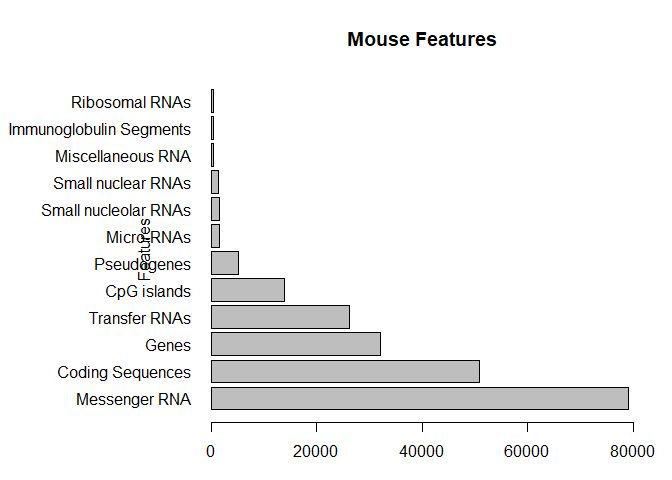
\includegraphics{Class_6_Homework_files/figure-latex/unnamed-chunk-2-3.pdf}


\end{document}
